\documentclass[tikz,border=0pt]{standalone}
\usepackage{graphicx}
\usepackage{xfp}
\usetikzlibrary{spy}

% ========================= 用户参数设置 =========================
\newcommand{\samplewidth}{1}                % 采样框宽度 (cm) 
\newcommand{\sampleheight}{1.6}             % 采样框高度 (cm) 
\newcommand{\magnificationfactor}{2}        % 放大倍数
\newcommand{\figurepath}{example-image}     % 图像文件路径
\newcommand{\linewidthmacro}{1.5pt}         % 设置线框线宽
\newcommand{\connectlinewidth}{1pt}         % 设置连接线线宽
% 设置采样框和放大框的位置
\newcommand{\spypointx}{0.51}               % 采样框中心 x 坐标
\newcommand{\spypointy}{0.5}                % 采样框中心 y 坐标
\newcommand{\spyviewerx}{0.75}              % 放大框中心 x 坐标
\newcommand{\spyviewery}{0.8}               % 放大框中心 y 坐标
% 如果希望去掉连接线,注释掉最后的 \draw 命令,也可以通过修改 \draw 命令来实现改变连接线为箭头等等

% ==== 自动计算放大框尺寸(单位为 cm) ====
\newcommand{\spywidth}{\fpeval{\samplewidth * \magnificationfactor}}   % 放大框宽度
\newcommand{\spyheight}{\fpeval{\sampleheight * \magnificationfactor}} % 放大框高度

\begin{document}
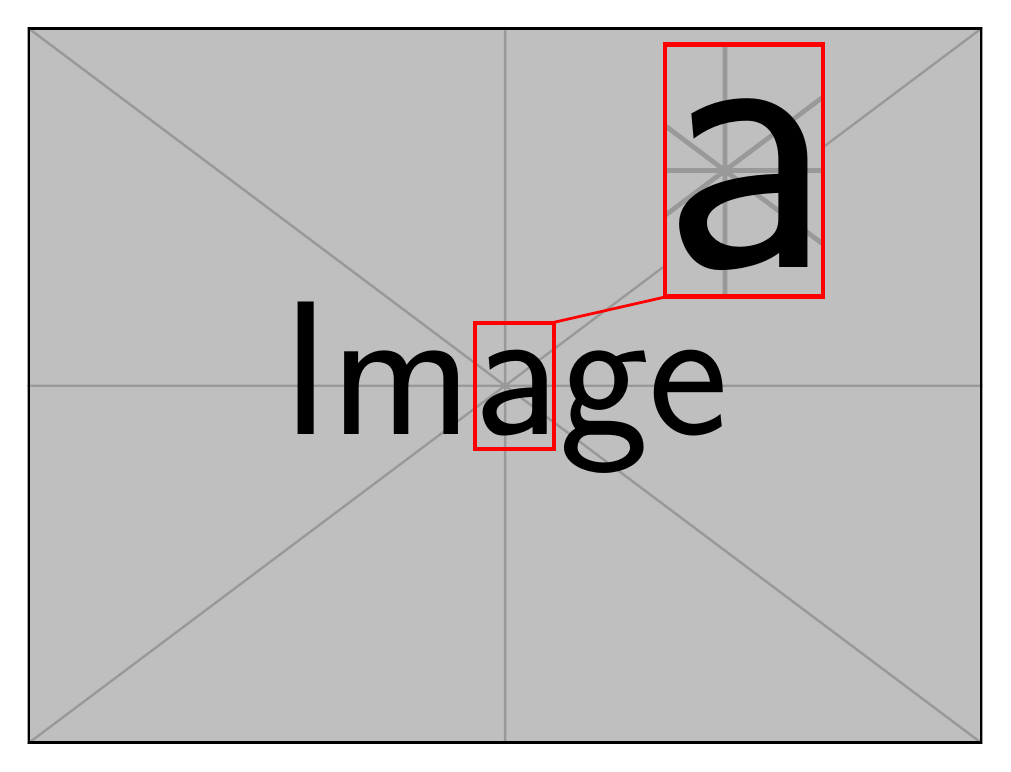
\begin{tikzpicture}[spy using outlines={
    rectangle, 
    magnification=\magnificationfactor, 
    every spy on node/.style={line width=\linewidthmacro, draw=red}, 
    every spy in node/.style={line width=\linewidthmacro, draw=red}
}]

    % ===== 原图 =====
    \node[anchor=south west, inner sep=0] (img) at (0,0)
        {\includegraphics[width=\textwidth]{{\figurepath}}};

    % ===== 坐标映射 =====
    \begin{scope}[x={(img.south east)}, y={(img.north west)}]
        \coordinate (spypoint) at (\spypointx,\spypointy);     % 采样点中心
        \coordinate (spyviewer) at (\spyviewerx,\spyviewery); % 放大框中心
    \end{scope}

    % ===== 放大框和采样框 =====
    \node[anchor=center, width=\samplewidth cm, height=\sampleheight cm, name=smallbox] at (spypoint) {};
    \node[anchor=center, width=\spywidth cm, height=\spyheight cm, name=bigbox] at (spyviewer) {};

    % ===== 放大视图 =====
    \spy[width=\spywidth cm, height=\spyheight cm] on (spypoint) in node[fill=none] at (spyviewer);

    % ===== 连接线 =====
    \draw[line width=\connectlinewidth, red] (smallbox.north east) -- (bigbox.south west);

\end{tikzpicture}
\end{document}